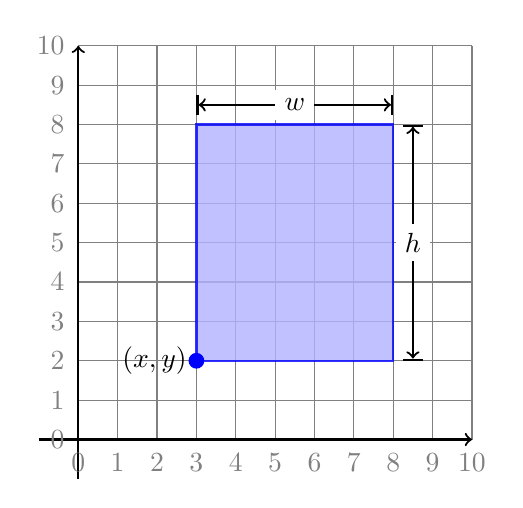
\begin{tikzpicture}[scale=.5]

  \def\gridsize{10}
  \def\Rw{5}
  \def\Rh{6}
  \def\Rx{3}
  \def\Ry{2}
  \draw[gray] (0, 0) grid (\gridsize, \gridsize);
  \draw[thick,->] (-1, 0) -- (\gridsize, 0);
  \draw[thick,->] (0, -1) -- (0, \gridsize);
  \draw[blue, thick, fill=blue!30, opacity=.8] (\Rx, \Ry) rectangle ++(\Rw, \Rh);
  \fill[blue] (\Rx, \Ry) circle (.2cm);
  \foreach\i in {0,...,{\gridsize}} {
      \node[gray, anchor=north] at (\i, -.1) {\i};
      \node[gray, anchor=east] at (-.1, \i) {\i};
  }
  \node[anchor=east] at (\Rx, \Ry) {\((x, y)\)};
  \draw[|<->|, thick] (\Rx + \Rw + 0.5, \Ry) -- node[fill=white] {\(h\)} ++(0, \Rh);
  \draw[|<->|, thick] (\Rx, \Ry + \Rh + 0.5) -- node[fill=white] {\(w\)} ++(\Rw, 0);


\end{tikzpicture}

